
%%% Local Variables:
%%% mode: latex
%%% End:

\def\dx{.5cm}
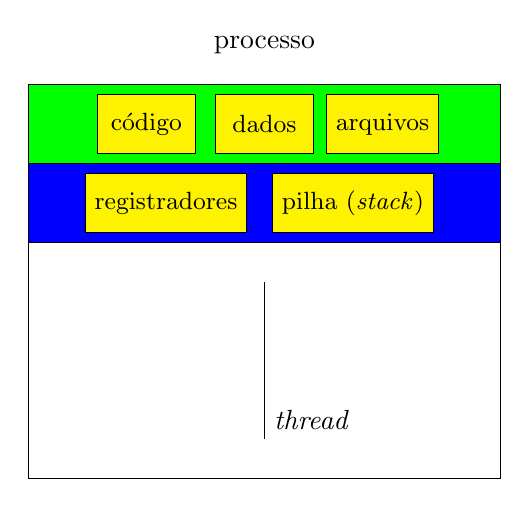
\begin{tikzpicture}[]
  \tikzset{resources/.style={minimum height=.75cm,minimum width=1.25cm,font=\small,fill=yellow,draw}}

  \node[fill=green,minimum width=6cm,minimum height=1cm,draw] at (0,0) (text) {};
  \node [above of=text] {processo};
  \node[resources] at (0,0) (data) {dados};
  \node[resources] (code) [left of=data,xshift=-\dx] {código};
  \node[resources] (files) [right of=data,xshift=\dx] {arquivos};

  \node[fill=blue,minimum width=6cm,minimum height=1cm,draw] (dynamic) [below of=text] {};
  \node[resources] (reg) [below of=code,xshift=0.5*\dx] {registradores};
  \node[resources] (stack) [right of=reg,xshift=2.75*\dx] {pilha (\emph{stack})};
  \node[minimum width=6cm,minimum height=5cm,draw] (threadsection) [below of=dynamic] {};
  \draw (0,-4*\dx) -- +(0,-2cm) node[anchor=south west] {\em thread};
\end{tikzpicture}
    